\section{Task 3: Symbol cutting for plain text, and the freeze}
\sectionmark{Task 3: Symbol cutting and the freeze}
\label{sec:t3}

\subsection{Purpose, conditions and criterion}

\begin{plain}{Task 3 at a glance}
\textbf{Purpose.} On the simulated photographs of 23 November the pipeline read lines of
mathematics far better than lines of ordinary text, whose letters were cut wrongly: thin
strokes broke, so that one letter became two pieces, and neighbouring letters touched, so that
two became one. This task finds out, on real photographs, why lines are misread; removes the
causes that can be removed without programming; hands the remaining ones to the project lead
with evidence; decides whether fractions remain part of what is demonstrated; and then
\term{freezes} the pipeline, so that the final measurement and the demonstration use one fixed
version.

\textbf{Before you begin.} Tasks~1 and~2 are complete, and the 20 development lines have been
photographed (Task~4, part~A, Section~\ref{sec:t4a}).

\textbf{Complete when.} (1)~Every development line that was misread has been assigned to a
kind of error. (2)~Every trial of a setting is recorded with its result, and was adopted or
rejected by the rule of Section~\ref{sec:trials}. (3)~The decision about fractions is recorded
with the figures on which it rests. (4)~The frozen version carries the tag \texttt{v1.0-rc1}.

\textbf{Time.} About two hours.
\end{plain}

\subsection{How a line is read, and how it can be misread}
\label{sec:kinds}

The pipeline reads a photograph in three stages, and each stage can fail in its own way.

\begin{enumerate}
\item \textbf{Cutting} (\term{segmentation}). Every pixel that is clearly darker than its
  surroundings is declared ink. Connected patches of ink are found, patches that belong
  together are joined (the dot and the stem of an \emph{i}, the two bars of an equals sign),
  and each resulting symbol receives a box.
\item \textbf{Recognition} (\term{classification}). The content of each box is scaled to a
  crop of $32 \times 32$ pixels and named by the neural network, which also states how
  confident it is.
\item \textbf{Layout.} From the names, sizes and positions of the boxes the program decides
  what is a superscript, a subscript, a numerator or a denominator, where words end, and which
  member of a group of look-alikes is meant (for example the letter o, the capital O or the
  digit 0), and writes the \LaTeX{} text.
\end{enumerate}

A fault in an early stage spoils the later ones: a letter that was cut into two pieces cannot
be named correctly, however good the network is. For this reason the first question about a
misread line is always at which stage it went wrong, and the review document of
Step~\ref{st:review} answers it at a glance, because it shows the boxes and the names
(Figure~\ref{fig:triage}). Table~\ref{tab:kinds} defines the kinds of error that this task
distinguishes.

\begin{figure}[H]
\centering
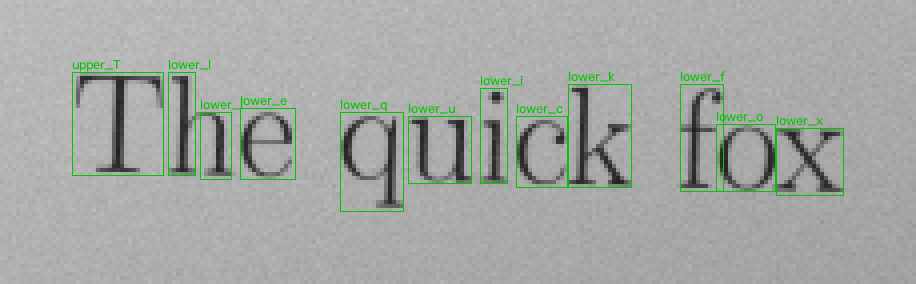
\includegraphics[width=0.86\linewidth]{img/triage_broken.png}\\[3pt]
{\small (a)}\\[5pt]
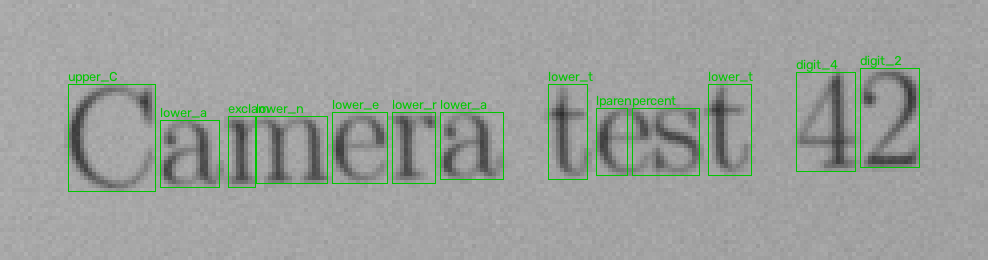
\includegraphics[width=0.92\linewidth]{img/triage_merged.png}\\[3pt]
{\small (b)}\\[5pt]
\begin{minipage}[b]{0.34\linewidth}\centering
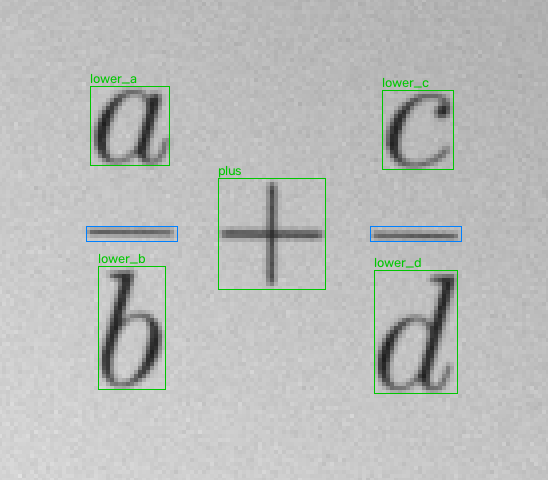
\includegraphics[height=3.6cm]{img/triage_ok.png}\\[3pt]{\small (c)}
\end{minipage}\hfill
\begin{minipage}[b]{0.38\linewidth}\centering
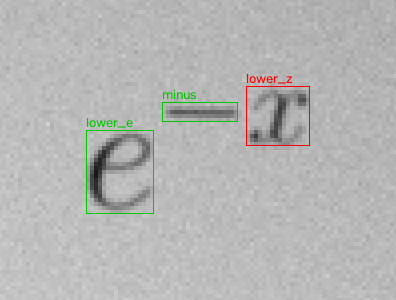
\includegraphics[height=2.6cm]{img/triage_recog.png}\\[3pt]{\small (d)}
\end{minipage}\hfill
\begin{minipage}[b]{0.24\linewidth}\centering
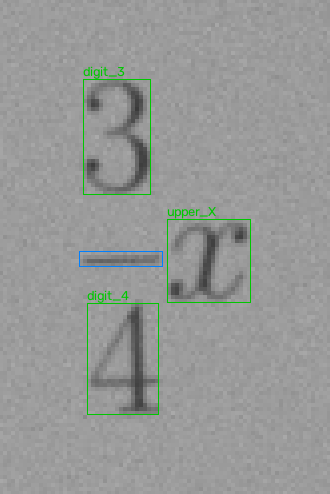
\includegraphics[height=3.6cm]{img/triage_layout.png}\\[3pt]{\small (e)}
\end{minipage}
\caption{Simulated photographs as the review document shows them, with the box and the name of
every symbol. (a)~A cutting error: the letter \emph{h} has broken into two boxes. (b)~Two
cutting errors: the \emph{m} is broken, and the letters \emph{e} and \emph{s} share boxes.
(c)~A line cut and named correctly; the bars of fractions are blue. (d)~A recognition error:
every symbol has one box, but the \emph{x} is named \emph{z}; the red box marks a symbol about
which the network was uncertain. (e)~A layout error: boxes and names are right, but the
\emph{x} was written as a superscript.}
\label{fig:triage}
\end{figure}

\begin{table}[H]
\centering
\begin{tabular}{C{1.0cm}L{2.5cm}L{7.6cm}}
\toprule
\hd{Code} & \multicolumn{1}{c}{\hd{Kind of error}} & \multicolumn{1}{c}{\hd{How it shows in the review document}} \\
\midrule
P & Photograph & The line is not wholly in the picture, a second line lies near the middle, a
  shadow or a bright spot crosses the line, or the picture is blurred by movement \\
C1 & Cutting: broken & One printed symbol has two or more boxes \\
C2 & Cutting: joined & Two or more printed symbols share one box \\
C3 & Cutting: lost or extra & A printed symbol has no box (usually a dot or a thin bar), or a box
  stands where nothing is printed \\
R & Recognition & Every symbol has exactly one box, but the name above a box is wrong \\
L & Layout & Boxes and names are right, but the \LaTeX{} is not: a wrong member of a look-alike
  group, a missing or extra space, a wrong superscript or subscript, a wrong fraction \\
\bottomrule
\end{tabular}
\caption{Kinds of error. When several apply to one line, the earliest stage counts: P before C,
C before R, R before L.}
\label{tab:kinds}
\end{table}

\subsection{The rule about the two sets of lines}

The 80 printed lines form two sets with different purposes. The 20 \term{development lines},
D01 to D20, may be examined as closely and as often as desired: every trial of this task is
judged on them. The 60 \term{test lines}, T01 to T60, measure the final accuracy and are
evaluated only at the gate of Section~\ref{sec:gate} and in Task~4. Until then, do not
evaluate them, do not open their review document, and do not choose a setting because of them.
A pipeline that has been adjusted to its own test lines reads those lines well and unknown
lines no better, and its measured accuracy would be worth nothing.

\subsection{Establish the baseline}

\step{Open the project in PowerShell}
% The opening sequence, written out in full. Input wherever a task may begin in a new window.
If a PowerShell window whose prompt begins with \texttt{(.venv)} is still open, use it and go
on to the next step. Otherwise open a new window (click \ui{Start}, type \code|powershell|,
click \ui{Windows PowerShell}) and give the two commands of the opening sequence in it.
\begin{ps}[Opening sequence, command 1 of 2]
cd C:\ee105\camera-to-latex
\end{ps}
\begin{ps}[Opening sequence, command 2 of 2]
.\.venv\Scripts\Activate.ps1
\end{ps}
\checkpoint{The prompt reads:}
\venvprompt


\step{Evaluate the development lines}\label{st:devbase}
\begin{ps}
python -m tools.eval_pipeline --split dev
\end{ps}
\begin{out}[Form of the output (the readings are the result of the measurement)]
ok D01 plain     expected Arduino Nano                 got Arduino Nano
-- D02 plain     expected Line 7: OK                   got ...
...
category   lines   exact     TER  compiles  s/line
plain         13     ...%    ...%    100.0%    ...
scripts        3     ...%    ...%    100.0%    ...
fractions      2     ...%    ...%    100.0%    ...
mixed          2     ...%    ...%    100.0%    ...
all           20     ...%    ...%    100.0%    ...

per-line results: C:\ee105\camera-to-latex\results\eval_dev_20261125_1410.csv
\end{out}
\checkpoint{The row \emph{all} reports 20 lines. If it reports fewer, photographs are missing
from \file{test\_set\bs images}: complete part~A of Task~4 first. Write down the names of the
lines that begin with \texttt{ok}; their number is the \emph{baseline}.}

\step{Produce the review document of the misread lines}\label{st:review}
Give this command directly after the evaluation, because the review program always describes
the most recent evaluation.
\begin{ps}
python -m tools.review_results --only-wrong
\end{ps}
\begin{out}
review: C:\ee105\camera-to-latex\results\review_dev_20261125_1410_wrong.pdf
\end{out}
\begin{ps}
explorer results
\end{ps}
In the Explorer window, double-click the file whose name begins with \file{review\_dev} and
ends with \file{\_wrong.pdf}. Each misread line occupies one row: at the left its photograph,
enlarged, with the boxes and names; at the right the expected line as it should be typeset, the
line as the pipeline read it (in orange), and both as \LaTeX{} text.
\checkpoint{The document shows one row for every line that the evaluation marked with
\texttt{-{}-}.}

\step{Assign every misread line to a kind of error}\label{st:triage}
For each row, compare the boxes with the printed symbols, then the names with the symbols, then
the two \LaTeX{} texts, and enter in Table~\ref{tab:triage} the first code of
Table~\ref{tab:kinds} that applies, with a few words that name the symbols concerned.

\begin{table}[H]
\centering
\begin{tabular}{C{1.3cm}C{1.3cm}L{8.2cm}}
\toprule
\hd{Line} & \hd{Code} & \multicolumn{1}{c}{\hd{What went wrong (symbols concerned)}} \\
\midrule
 & & \\[5pt] \cmidrule{1-3}
 & & \\[5pt] \cmidrule{1-3}
 & & \\[5pt] \cmidrule{1-3}
 & & \\[5pt] \cmidrule{1-3}
 & & \\[5pt] \cmidrule{1-3}
 & & \\[5pt] \cmidrule{1-3}
 & & \\[5pt] \cmidrule{1-3}
 & & \\[5pt] \cmidrule{1-3}
 & & \\[5pt] \cmidrule{1-3}
 & & \\[5pt]
\bottomrule
\end{tabular}
\caption{Triage of the misread development lines. Example of an entry: \emph{D03, C2, the
letters T and r share a box.}}
\label{tab:triage}
\end{table}
\checkpoint{Every misread line has a code. Count the lines of each code; the counts decide
which of the following subsections apply.}

\subsection{Errors of the photograph (code P)}

\step{Take the faulty photographs again}
Set up the line position as in part~A of Task~4, and give the capture command with the names of
the lines in place of the placeholder, separated by commas and without spaces:
\begin{center}
\mbox{\footnotesize\texttt{python -m pipeline.capture -{}-series test\_set\textbackslash{}images -{}-names "}\ph{NAMES}\texttt{"}}
\end{center}
\begin{out}[Example only: the command for retaking D07 and D12]
python -m pipeline.capture --series test_set\images --names "D07,D12"
\end{out}
Then repeat Steps~\ref{st:devbase} to~\ref{st:triage}. The new result is the baseline.
\checkpoint{No line carries the code P any longer.}

\subsection{Cutting errors (codes C1, C2 and C3)}
\label{sec:cutting}

Cutting errors have three possible causes, which are examined in this order: letters that are
too small or not sharp; uneven or weak light; and settings of the cutting stage that do not
suit the real photographs.

\step{Confirm the size and sharpness of the letters}
Look up the width $W$ of line T39 in the record of Task~1.
\checkpoint{$W$ lies between 280 and 300 pixels, and the trial was judged sharp. If not, the
calibration of the line position is repeated, and all 80 lines are photographed again, before
anything else is tried: no setting can restore detail that the photograph does not contain.}

\rationale{In simulated photographs read with the fallback classifier, the number of lines read
exactly rose from 57 of 80 at a capital height of 24 pixels to 63 at 28 pixels and 65 at 30
pixels, and that of the nine lines of text from one to four to six
(Table~\ref{tab:simsettings}, first row). No setting had an effect of comparable size.}

\step{Examine the light}
Open three development photographs that show cutting errors (\code|explorer test_set\images|,
then double-click) and compare the paper to the left and to the right of the line.
\checkpoint{The paper is a similar gray on both sides, the ink is clearly darker than the paper
everywhere, and no part of the line lies in a shadow. If one side is much darker, correct the
lamps as in Task~1 and take the affected photographs again.}

\subsubsection*{Trials of settings}
\label{sec:trials}

The cutting stage is governed by a few settings of \file{config.py}. Table~\ref{tab:candidates}
lists the four that are worth a trial and says which kind of error each might reduce.
Table~\ref{tab:simsettings} shows what the same settings, and some others, did in simulation.
Its message is sobering and should be kept in mind: no setting improved the reading at every
size, and several settings that look plausible did serious harm. It is therefore a legitimate
and likely outcome of this subsection that every trial is rejected and the settings remain as
they are.

\begin{table}[H]
\centering
\begin{tabular}{L{3.0cm}C{1.2cm}C{1.2cm}L{5.4cm}}
\toprule
\multicolumn{1}{c}{\hd{Setting}} & \hd{Now} & \hd{Trial} & \multicolumn{1}{c}{\hd{Intended effect}} \\
\midrule
\texttt{THRESH\_WEAK\_C} & 5 & 3 & Faint ink that touches certain ink is kept more readily;
  may mend broken strokes (C1) \\
\texttt{THRESH\_C} & 10 & 8 & A pixel needs to be less dark to count as ink; may mend broken
  strokes and lost dots (C1, C3) \\
\texttt{THRESH\_C} & 10 & 12 & A pixel must be darker to count as ink; may separate letters
  that touch, and remove boxes on bare paper (C2, C3) \\
\texttt{THRESH\_BLOCK} & 31 & 41 & The surroundings with which a pixel is compared are larger;
  may help when letters are large and their strokes thick (C1) \\
\bottomrule
\end{tabular}
\caption{Candidate settings for the trials. Each is tried alone, starting from the baseline.}
\label{tab:candidates}
\end{table}

\begin{table}[H]
\centering
\begin{tabular}{L{4.2cm}C{1.7cm}C{1.7cm}C{1.7cm}}
\toprule
\multicolumn{1}{c}{\hd{Setting changed}} & \hd{24 px} & \hd{28 px} & \hd{30 px} \\
\midrule
None (the present settings) & 57 & 63 & 65 \\
\texttt{THRESH\_WEAK\_C = 3} & 60 & 61 & 65 \\
\texttt{THRESH\_C = 8} & 56 & 62 & 64 \\
\texttt{THRESH\_C = 12} & 57 & 63 & 65 \\
\texttt{THRESH\_BLOCK = 41} & 62 & 61 & 65 \\
\midrule
\texttt{THRESH\_BLOCK = 21} & 50 & 55 & 62 \\
\texttt{THRESH\_WEAK\_C = None} & 49 & 53 & 61 \\
\texttt{CLOSE\_KSIZE = 2} & 53 & 59 & 61 \\
\texttt{BLUR\_KSIZE = 5} & 49 & 53 & 56 \\
\texttt{BLUR\_KSIZE = 0} & 16 & 15 & 16 \\
\texttt{SPACE\_GAP = 0.5} & 56 & 60 & 60 \\
\texttt{LAYOUT\_LEVEL = 2} & 44 & 50 & 52 \\
\bottomrule
\end{tabular}
\caption{Simulation: lines read exactly, of 80, at three capital heights, with one setting
changed at a time (fallback classifier, simulated photographs, 24 November). The settings
below the middle rule did harm at every size and are not to be tried.}
\label{tab:simsettings}
\end{table}

\step{Prepare two sets of simulated photographs at the calibrated size}\label{st:sims}
The simulated photographs of the quick start have capitals of 24 pixels. These two commands
produce 80 photographs each at 29 pixels, the middle of the calibrated range, with different
random tilts, lighting and noise.
\begin{ps}
python -m tools.make_test_lines --render --cap-px 29 --out data\sim0
\end{ps}
\begin{ps}
python -m tools.make_test_lines --render --cap-px 29 --seed 1 --out data\sim1
\end{ps}
\begin{out}[After the second command]
80 fake photos (29 px capitals) -> data\sim1
\end{out}
Now measure the baseline on both sets. The option \code|--no-compile| omits the check that each
reading compiles, which is not needed here and takes most of the time; the column
\emph{compiles} of the table then shows \emph{nan}. The option \code|--quiet| prints the table
alone.
\begin{ps}
python -m tools.eval_pipeline --images data\sim0 --split all --no-compile --quiet
\end{ps}
\begin{ps}
python -m tools.eval_pipeline --images data\sim1 --split all --no-compile --quiet
\end{ps}
\checkpoint{For each of the two tables, multiply the percentage in the row \emph{all} by 80 to
obtain the number of lines read exactly (78.8\,\% of 80 lines is 63 lines), and enter the sum
of the two numbers in the row \emph{baseline} of Table~\ref{tab:trialrec}.}

\step{Carry out one trial}\label{st:trial}
A trial changes a single setting and compares the result with the baseline.
\begin{enumerate}
\item Change the setting to its trial value by the method of Section~\ref{sec:setting}, and
  check that the file is valid (Step~\ref{st:valid}).
\item Evaluate the development lines:
\begin{ps}
python -m tools.eval_pipeline --split dev
\end{ps}
\item Compare the list with that of the baseline, line by line. Count the lines that are now
  \texttt{ok} and were not (\emph{gained}), and the lines that were \texttt{ok} and are no
  longer (\emph{lost}).
\item If no line was gained, or more were lost than gained, the trial has failed: go to item~6.
\item Otherwise evaluate the two simulated sets with the two commands at the end of
  Step~\ref{st:sims}, and add up the lines read exactly.
\item Enter the trial in Table~\ref{tab:trialrec}, and apply the rule below.
\end{enumerate}

\begin{plain}{The rule of adoption}
A setting is adopted only if \emph{both} conditions hold: on the 20 real development
photographs it gains at least two lines and loses none; and on the 160 simulated photographs it
reads at least as many lines as the baseline.
\end{plain}

\rationale{The pipeline contains no element of chance, so that the same photographs always give
the same reading, and a line gained on these photographs is a fact. What remains uncertain is
whether the gain will hold for other photographs. Twenty lines cannot settle that
(Section~\ref{sec:stat}); the 160 simulated photographs serve as a second, independent
witness. The rule is deliberately strict, because an adopted setting that does harm is
discovered only in the demonstration.}

\step{After a rejected trial: restore the settings}
\begin{ps}
git restore config.py
\end{ps}
\checkpoint{The command prints nothing. The file is again as it was at the last commit.}

\step{After an adopted trial: record the setting}
\begin{ps}
git add config.py
\end{ps}
\begin{ps}
git commit -m "Adopt a cutting setting after a trial on the development lines"
\end{ps}
The adopted state is now the baseline for any further trial: its list of \texttt{ok} lines and
its number of simulated lines replace the earlier ones.
\checkpoint{The second command printed a line that begins with \texttt{[main}.}

\begin{table}[H]
\centering
\begin{tabular}{L{3.4cm}C{1.45cm}C{1.1cm}C{1.95cm}C{2.6cm}}
\toprule
\multicolumn{1}{c}{\hd{Setting and value}} & \hd{Gained} & \hd{Lost} & \hd{Simulated, of 160} & \hd{Adopted?} \\
\midrule
Baseline & -- & -- & & -- \\
 & & & & \cbox\ yes\ \ \cbox\ no \\
 & & & & \cbox\ yes\ \ \cbox\ no \\
 & & & & \cbox\ yes\ \ \cbox\ no \\
 & & & & \cbox\ yes\ \ \cbox\ no \\
\bottomrule
\end{tabular}
\caption{Record of the trials. \emph{Gained} and \emph{lost} refer to the 20 development
lines.}
\label{tab:trialrec}
\end{table}

\begin{caution}[Settings that are not to be changed]
The settings below the middle rule of Table~\ref{tab:simsettings} are left alone. In
particular, \texttt{BLUR\_KSIZE = 0} looks like a way to obtain sharper letters and destroys
the reading almost completely, because the noise of the sensor then turns into ink. The
orientation settings of Task~1 and all settings of the classifier and of the layout are not
part of these trials either.
\end{caution}

\subsection{Recognition and layout errors (codes R and L)}
\label{sec:rl}

Errors of these two kinds cannot be removed by a setting. They are recorded here, so that the
project lead can decide what to do about them and so that the final report can describe them.

\step{Describe the recognition errors}
For every line with the code R, note which symbol was mistaken for which, and compare with the
list \emph{most common confusions} of Task~2 (Step~\ref{st:after}).
\checkpoint{The record states whether the confusions of whole lines are the same pairs that
dominate the confusions of single crops. If they are, a second round of sheet photographs
(Section~\ref{sec:round2}) is the remedy that needs no programming, and the lead decides
whether the time allows it. A very small symbol, such as a superscript, that is confused with a
similar one is to be expected at this resolution, and is reported as a limit of the method.}

\step{Describe the layout errors}
For every line with the code L, note the expected and the obtained \LaTeX{} text.
\checkpoint{The record lists them. Typical cases are a letter after a fraction that was taken
for a superscript, a colon read as a semicolon, and a capital letter chosen in place of the
small one of the same shape.}

\subsubsection*{Changes to the program (project lead only)}

A change to the Python code of the pipeline can do what no setting can, for example cut a wide
box at its thinnest place when the network is uncertain, or join the parts of a per cent sign.
It can also break what works. A change is therefore made on a separate \term{branch} of the
repository and joins the main line only if it passes three checks: the automatic tests, the
development lines under the rule of adoption, and the simulated photographs.
\begin{ps}[Start a branch for the change]
git switch -c fix-cutting
\end{ps}
After the change has been written:
\begin{ps}[Check 1: the automatic tests]
python -m pytest -q
\end{ps}
\begin{ps}[Check 2: the development lines]
python -m tools.eval_pipeline --split dev
\end{ps}
Check~3 consists of the two commands at the end of Step~\ref{st:sims}. If all three checks
pass, record the change on the branch, join the branch to the main line, and upload:
\begin{ps}
git commit -a -m "Improve the cutting of symbols in text lines"
\end{ps}
\begin{ps}
git switch main
\end{ps}
\begin{ps}
git merge fix-cutting
\end{ps}
\begin{ps}
git push
\end{ps}
If a check fails and cannot be repaired in the time available, the branch is simply left
behind: \cmd{git stash} sets the unfinished change aside, and \cmd{git switch main} returns to
the version that works.

\subsection{The gate: do fractions remain?}
\label{sec:gate}

The project plan contains a gate for 25 November: lines with fractions are read exactly in at
least 60\,\% of cases, or the support for fractions is withdrawn from what is handed in. The
gate is the first of the two occasions on which the test lines are evaluated.

\step{Evaluate the test lines once}\label{st:gaterun}
All trials are finished, and the settings are those that will be frozen.
\begin{ps}
python -m tools.eval_pipeline
\end{ps}
Without the option \code|--split| the command evaluates the 60 test lines.
\begin{out}[Form of the output: the table at the end]
category   lines   exact     TER  compiles  s/line
plain         25     ...%    ...%    ...%    ...
scripts       20     ...%    ...%    ...%    ...
fractions     10     ...%    ...%    ...%    ...
mixed          5     ...%    ...%    ...%    ...
all           60     ...%    ...%    ...%    ...
\end{out}
\checkpoint{The row \emph{all} reports 60 lines. Enter the five rows in the record
(Table~\ref{tab:t3record}), as counts: 80.0\,\% of 25 lines is 20 lines.}

\step{Decide}\label{st:gatedecide}
\begin{itemize}
\item \textbf{Six or more of the ten fraction lines were read exactly.} The target is met.
  Fractions remain, and the demonstration includes a fraction. Go to Section~\ref{sec:freeze}.
\item \textbf{Five or fewer were read exactly.} The target is missed. Fractions are not
  demonstrated, and the report states the result as measured. Whether the support is also
  switched off depends on the next step.
\end{itemize}
With ten lines the measurement is coarse: its standard error is 15 points
(Table~\ref{tab:stat}). The gate is nevertheless applied as it was agreed; the report gives the
count and names the uncertainty.

\step{Only if the target was missed: compare with fractions switched off}
Switching fractions off cannot help the fraction lines themselves, which are then certainly
misread. It is worth while only if the fraction logic damages \emph{other} lines, for example
by taking a minus sign for the bar of a fraction. Set \code|LAYOUT_LEVEL| to \code|2| by the
method of Section~\ref{sec:setting} and evaluate the same photographs again:
\begin{ps}
python -m tools.eval_pipeline --no-compile --quiet
\end{ps}
Compare the rows \emph{plain} and \emph{scripts} with those of Step~\ref{st:gaterun}. The
photographs are the same, so any difference is caused by the setting alone.
\begin{itemize}
\item If level~2 reads more plain and script lines in total, keep \code|LAYOUT_LEVEL = 2|:
  fractions are switched off for the hand-in, and the rows of this second evaluation are the
  ones that count.
\item Otherwise restore level~3 with the command below. Fractions stay enabled, because
  switching them off would gain nothing, but they are neither demonstrated nor claimed.
\end{itemize}
\begin{ps}[Only if level 3 is to be restored]
git restore config.py
\end{ps}
\checkpoint{The decision, and the counts of plain and script lines at both levels, are entered
in the record.}

\rationale{In simulation, switching fractions off did not help a single line of the other
categories at any size. It cost every fraction line and three others, which need the same part
of the program: the sum with its limits above and below (T45), a square root (T56) and a line
that contains a fraction (T60); see the last row of Table~\ref{tab:simsettings}. The comparison
is nevertheless made on the real photographs, because only they can show whether the fraction
logic misfires there.}

\subsection{The freeze}
\label{sec:freeze}

From the freeze onwards, neither the settings nor the program nor the classifier is changed,
except to repair a defect that would prevent the demonstration; after any such repair the final
measurement of Task~4 is repeated, and both results are reported.

\step{Check, record and mark the frozen version}\label{st:freeze}
\begin{ps}
python -m pytest -q
\end{ps}
\begin{ps}
git status --short
\end{ps}
\checkpoint{The tests pass. The second command prints nothing, or only the line
\texttt{\ M config.py}. If it lists other files, something has been left unrecorded: the
photographs of Task~4, part~A, are recorded by the last step of that part; for anything else,
ask the lead before continuing.}
If \file{config.py} is listed, record it:
\begin{ps}
git add config.py
\end{ps}
\begin{ps}
git commit -m "Settings frozen for the demonstration"
\end{ps}
Then upload the main line, and attach a \term{tag}, a permanent name for exactly this version:
\begin{ps}
git push
\end{ps}
\begin{ps}
git tag -a v1.0-rc1 -m "Frozen for the final measurement and the demonstration"
\end{ps}
\begin{ps}
git push origin v1.0-rc1
\end{ps}
\begin{ps}
git rev-parse --short HEAD
\end{ps}
\checkpoint{The last command prints seven letters and digits, the short name of the frozen
commit. Enter it in the record. The tag is visible on the GitHub page of the repository under
\emph{Tags}.}

\step{Fill in the record}
\begin{table}[H]
\centering
\begin{tabular}{L{7.2cm}C{4.0cm}}
\toprule
\multicolumn{1}{c}{\hd{Quantity}} & \hd{Value} \\
\midrule
Development lines read exactly at the baseline (of 20) & \\
Misread lines by kind: P; C1; C2; C3; R; L & \\
Settings adopted (name and value), or \emph{none} & \\
Development lines read exactly at the freeze (of 20) & \\
Simulated lines read exactly at the freeze (of 160) & \\
Gate, plain lines read exactly (of 25) & \\
Gate, script lines (of 20) & \\
Gate, fraction lines (of 10) & \\
Gate, mixed lines (of 5) & \\
Gate, all lines (of 60) & \\
Plain and script lines at level 2, if compared (of 45) & \\
\texttt{LAYOUT\_LEVEL} at the freeze; fractions demonstrated? & \\
Short name of the frozen commit; date & \\
\bottomrule
\end{tabular}
\caption{Record of Task 3.}
\label{tab:t3record}
\end{table}
